
	{The control unit is composed of the FSM and the 4:16 Decoder, operating in tandem to form an integrated control mechanism. Subsequent elucidation on the interworking of these elements follows.}

	\begin{figure}[H]
		\centering
		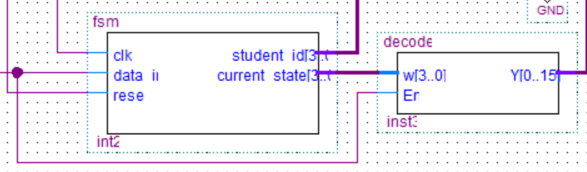
\includegraphics[width=10cm]{Pictures/ControlUnit.png}
		\caption{{Block Diagram for the Conrol Unit}}
		\label{}
	\end{figure}

\subsection{{Finite State Machine}}

	\subsubsection{{Description}}
	
		{The Mealy 9-state finite state machine is designed to act as a counter aligned with the digits of the student ID. With each rising edge of the clock signal, the machine transitions to the next state, effectively incrementing the count and progressing through the student ID digits.}
			
		{This synchronized mechanism ensures accurate counting, reflecting the sequential nature of the student ID. The machine's output is dynamically influenced by both the current state and the input, creating a responsive counter system tailored to the student ID's numerical representation.}
	
	\subsubsection{{Truth Table}}
	
		{The presented truth table delineates that under conditions where the clock signal undergoes a rising edge and the dataIn is assigned as 1, the output transitions to the subsequent state.}
		
		{Conversely, if these criteria are not met, the output persists in the current state. Notably, individual states are numerically designated, and in this context, they correspond to the assigned student number (501209136).}

		\begin{table}[H]
			\centering
			\begin{tabular}{|c|c|c|}
			\hline
			\hline
				\textit{Current State} & \textit{Next State (DataIn = 1 \& Clock = 1)} & \textit{Decimal Output} \\ 
				\hline
				\hline
				0000 & 0101 & 5 \\ \hline
				0001 & 0000 & 0 \\ \hline
				0010 & 0001 & 1 \\ \hline
				0011 & 0010 & 2 \\ \hline
				0100 & 0000 & 0 \\ \hline
				0101 & 1001 & 9 \\ \hline
				0110 & 0001 & 1 \\ \hline
				0111 & 0011 & 3 \\ \hline
				1000 & 0110 & 6 \\ \hline
			\hline
			\end{tabular}
		\end{table}
	
	\subsubsection{{Block Diagram}}
	
		{Figure \ref{FSM} depicts a block diagram characterized by three inputs and two outputs. The inputs encompass the clock signal, the preceding state, and the reset signal, where activation of the reset signal results in a transition to the initial state.}
		
		{The Finite State Machine (FSM) remains in its current state or advances to the subsequent state based on the interplay between dataIn and the clock signal. The output features both the student ID and the prevailing state, with the former directly routed to the display and the latter directed to the 4:16 decoder.}

		\begin{figure}[H]
			\centering
			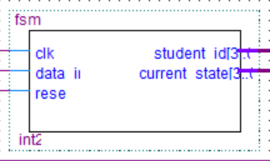
\includegraphics[width=10cm]{Pictures/FSM.png}
			\caption{{Block Diagram for the Mealy Finite State Machine}}
			\label{FSM}
		\end{figure}
	
	\subsubsection{{Timing Diagram}}
	
		{The timing diagram illustrates that the transition to the next state occurs when the clock signal experiences a rising edge, concurrently with the presence of dataIn. In the absence of these conditions, the system maintains its current state.}

		\begin{figure}[H]
			\centering
			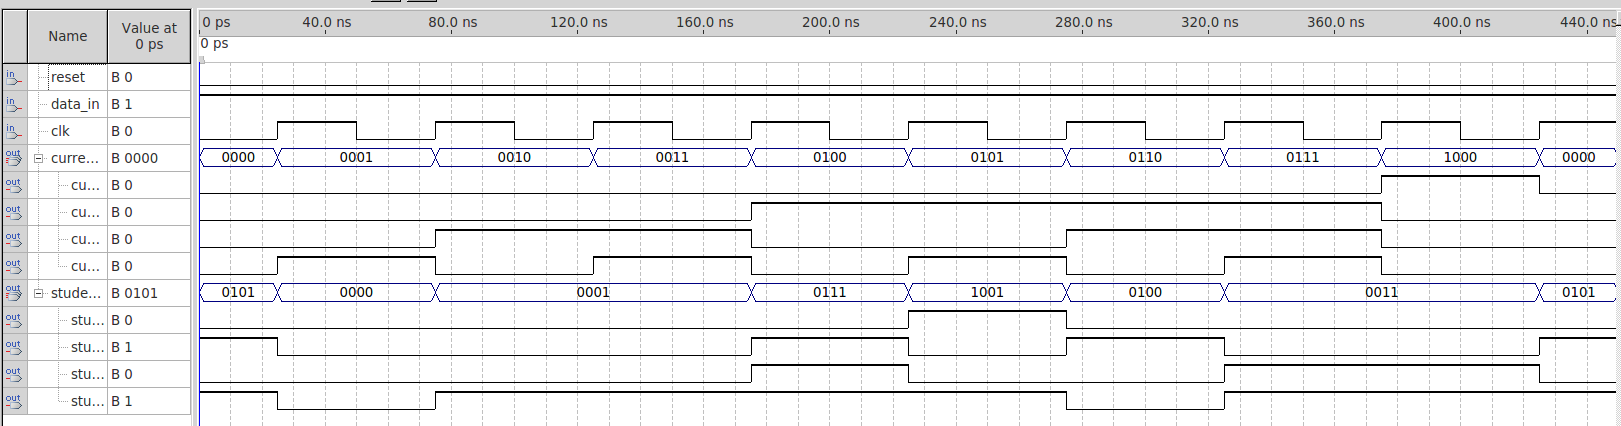
\includegraphics[width=15cm]{Pictures/FSMWaveForm.png}
			\caption{{Timing Diagram for the Mealy Finite State Machine}}
			\label{}
		\end{figure}

\subsection{{4:16 Decoder}}

	\subsubsection{{Description}}
	
		{The 4:16 decoder, modeled after Figure 3 in Lab6\_Manual, is derived from 3:8 decoders with modifications for a 4:16 configuration. Activated by an enable signal from the FSM, it decodes the current state, selecting one of the 16 outputs directed to the ALU Core. This decoder is implemented using two 3:8 decoders, effectively managing state decoding and streamlining the transition from 3:8 to 4:16 functionality.}
	
	\subsubsection{{Truth Table}}
	
		\begin{table}[H]
    			\centering
    			\begin{tabular}{|c|c|c|c|c|c|}
    			\hline
    			\hline
        			\textit{En} & $S_3$ & $S_2$ & $S_1$ & $S_0$ & $O(S_0, S_1, S_2, S_3, En)$ \\         			
        			\hline
        			\hline
        			1 & 0 & 0 & 0 & 0 & 0000000000000001 \\
        			\hline 
        			1 & 0 & 0 & 0 & 1 & 0000000000000010 \\ 
        			\hline 
        			1 & 0 & 0 & 1 & 0 & 0000000000000100 \\ 
        			\hline 
        			1 & 0 & 0 & 1 & 1 & 0000000000001000\\ 
        			\hline 
        			1 & 0 & 1 & 0 & 0 & 0000000000010000 \\ 
        			\hline 
        			1 & 0 & 1 & 0 & 1 & 0000000000100000 \\ 
        			\hline 
        			1 & 0 & 1 & 1 & 0 & 0000000001000000 \\ 
        			\hline 
        			1 & 0 & 1 & 1 & 1 & 0000000010000000 \\ 
        			\hline 
       				1 & 1 & 0 & 0 & 0 & 0000000100000000 \\ 
        			\hline 
        			1 & 1 & 0 & 0 & 1 & 0000001000000000 \\ 
        			\hline 
        			1 & 1 & 0 & 1 & 0 & 0000010000000000 \\ 
        			\hline 
        			1 & 1 & 0 & 1 & 1 & 0000100000000000 \\ 
        			\hline 
        			1 & 1 & 1 & 0 & 0 & 0001000000000000 \\ 
        			\hline 
        			1 & 1 & 1 & 0 & 1 & 0010000000000000 \\ 
        			\hline 
        			1 & 1 & 1 & 1 & 0 & 0100000000000000 \\ 
        			\hline 
        			1 & 1 & 1 & 1 & 1 & 1000000000000000 \\ 
        			\hline
        			\hline
    			\end{tabular}
    			\caption{Truth Table for the 4:16 Decoder}
			\end{table}
	
	\subsubsection{{Block Diagram}}
	
		\begin{figure}[H]
			\centering
			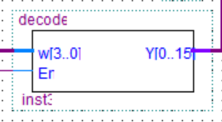
\includegraphics[width=10cm]{Pictures/decoder.png}
			\caption{{Block Diagram for the 4:16 Decoder}}
			\label{}
		\end{figure}
	
	\subsubsection{{Timing Diagram}}
	
		\begin{figure}[H]
			\centering
			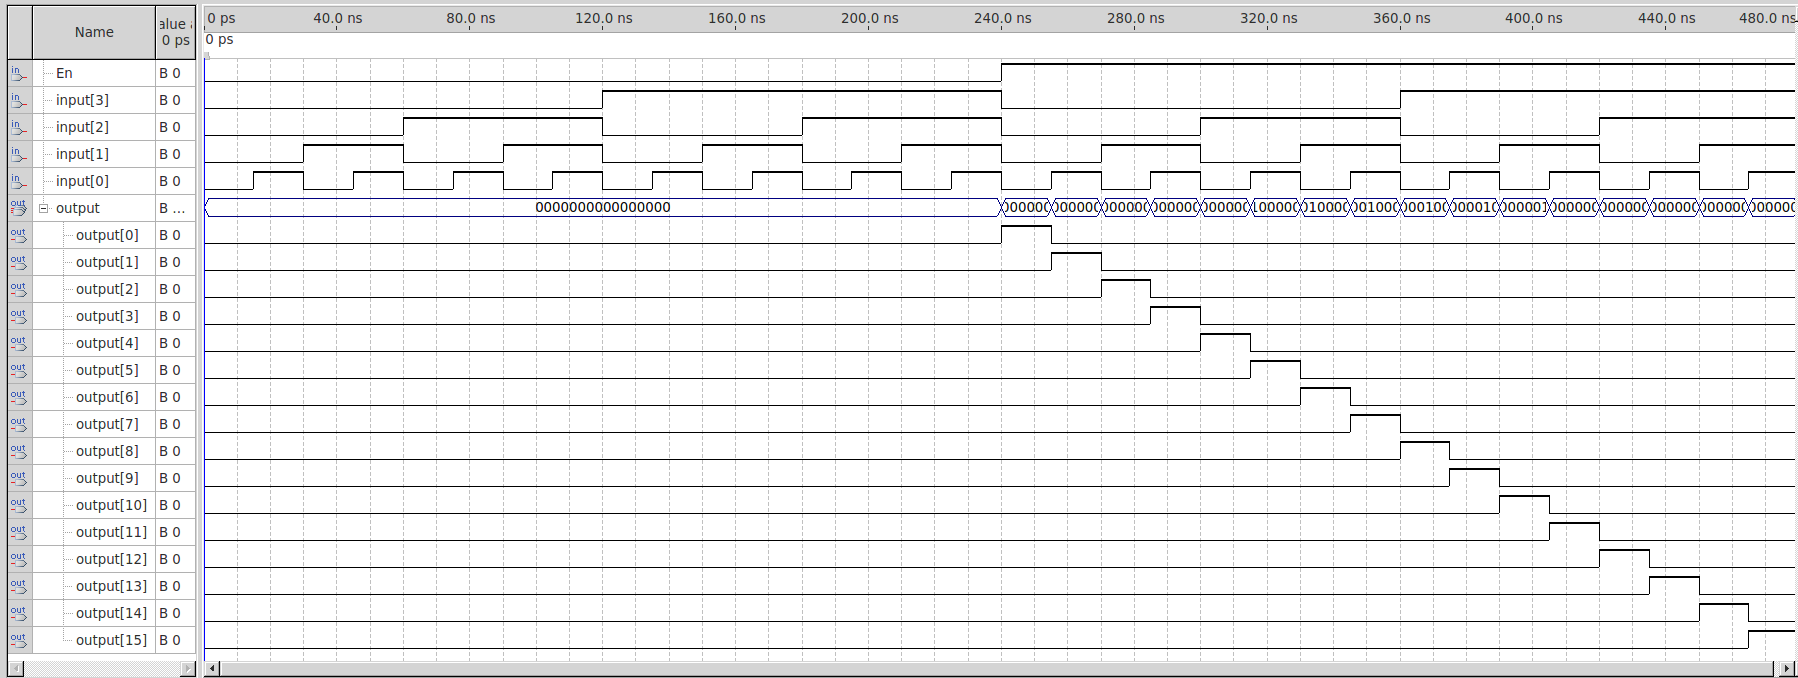
\includegraphics[width=15cm]{Pictures/DecoderWaveForm.png}
			\caption{{Timing Diagram for the 4:16 Decoder}}
			\label{}
		\end{figure}

